\let\lesson\undefined
\newcommand{\lesson}{\phantomlesson{Bài 20: Mạch dao động}}
\chapter[Cấu tạo và nguyên tắc của mạch dao động]{Cấu tạo và nguyên tắc của mạch dao động}
\section{Lý thuyết}
\subsection {Mạch dao động}
\begin{center}
	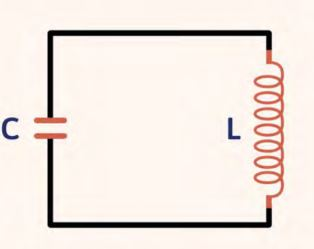
\includegraphics[scale=0.5]{../figs/4-1-1.JPG}
\end{center}
\begin{itemize}
	\item Gồm một tụ điện có điện dung $C$ mắc với một cuộn cảm có độ tự cảm $L$ thành mạch kín.
	\item Nếu điện trở của mạch rất nhỏ, coi như bằng không, thì mạch là một mạch dao động lý tưởng.
\end{itemize}
\subsection{Sự biến thiên điện tích và cường độ dòng điện trong mạch dao động lí tưởng}
Điện tích $q$ của một bản tụ điện và cường độ dòng điện $i$ trong mạch dao động biến thiên điều hòa theo thời gian, $i$ sớm pha $\dfrac{\pi}{2} $ so với $q$.
\begin{equation}
	q=q_0\cos(\omega t +\varphi)\ \text{C}, 
\end{equation}
\begin{equation}
	i=\frac{dq}{dt}=I_0 \cos(\omega t +\varphi+ \frac{\pi}{2})\ \text{A},
\end{equation}
trong đó: $I_0=q_0\omega, \omega =\dfrac{1}{\sqrt {LC}}$.
\subsection {Dao động điện từ tự do}
Sự biến thiên điều hòa theo thời gian của điện tích $q$ của một bản tụ điện và cường độ dòng điện $i$ (hoặc cường độ điện trường $\vec{E}$ và cảm ứng từ $\vec{B}$) trong mạch dao động được gọi là dao động điện từ tự do.
\subsection {Chu kì và tần số dao động riêng của mạch dao đông}
\begin{equation}
	T=2\pi \sqrt {LC},
\end{equation}
\begin{equation}
	f=\frac{1}{2\pi\sqrt {LC}},
\end{equation}
trong đó:
\begin{itemize}
	\item $L$: Độ tự cảm của cuộn dây ($\text{H}$);
	\item $C$: Điện dung của tụ điện ($\text{F}$);
	\item $T$: Chu kì dao động ($\text{s}$);
	\item $f$: Tần số dao động riêng của mạch dao động ($\text{Hz}$).
\end{itemize}
\subsection {Năng lượng điện từ}
\begin{itemize}
	\item Tổng năng lượng điện trường trong tụ điện và năng lượng từ trường trong cuộn cảm của mạch gọi là năng lượng điện từ.\\
	\begin{equation}
		W=W_{\text{đ}}+W_{t}=\frac{1}{2}Cu^2+\frac{1}{2}Li^2
	\end{equation}
	\item Nếu không có sự tiêu hao năng lượng thì năng lượng điện từ trong mạch sẽ được bảo toàn.
	\begin{equation}
		W=W_\text{đ max}=W_\text{t max}=\dfrac{1}{2}CU^2_0=\dfrac{1}{2}LI^2_0
	\end{equation}
\end{itemize}
\section{Mục tiêu bài học - Ví dụ minh họa}
\begin{dang}{Xác định chu kỳ, tần số, điện tích của mạch dao động}
	\viduii{2}{
		
		Mạch dao động LC lí tưởng gồm cuộn cảm có độ tự cảm $L = \SI{2}{mH}$ và tụ điện có điện dung $C = \SI{2}{pF}$. Tần số dao động của mạch gần bằng
		\begin{mcq}(4)
			\item $\SI{1}{MHz}$. 
			\item $\SI{2,5}{MHz}$. 
			\item $\SI{1}{kHz}$. 
			\item $\SI{2,5}{kHz}$. 
		\end{mcq}
	}
	{	\begin{center}
			\textbf{Hướng dẫn giải}
		\end{center}
		
		
		Tần số dao động riêng của mạch cho bởi
		
		$$f = \dfrac{1}{2\pi \sqrt{LC}} = \SI{2,5}{MHz}.$$
		
		\textbf{Đáp án: B.}
		
		
		\begin{center}
			\textbf{Câu hỏi tương tự}
		\end{center}
		
		Một mạch dao động gồm một cuộn cảm có độ tự cảm $L = \SI{1}{mH}$ và một tụ điện có điện dung là $C = \SI{0,1}{\mu F}$. Tần số riêng của mạch có giá trị nào?
		
		\textbf{Đáp án:} $f = \text{1,6}\cdot 10^4\ \text{Hz}$.
	}
	\viduii{2}{
		
		Mạch dao động điện từ lí tưởng gồm cuộn dây thuần cảm có độ tự cảm L và tụ điện có điện dung C. Khi tăng điện dung của tụ điện lên 9 lần thì chu kì dao động riêng của mạch
		\begin{mcq}(2)
			\item tăng lên 9 lần. 
			\item tăng lên 3 lần. 
			\item giảm đi 9 lần. 
			\item giảm 3 lần. 
		\end{mcq}
	}
	{	\begin{center}
			\textbf{Hướng dẫn giải}
		\end{center}
		
		Ban đầu, chu kì dao động riêng của mạch cho bởi công thức 
		
		$$T = 2\pi \sqrt{LC}.$$
		
		Lúc sau, chu kì dao động riêng của mạch cho bởi công thức 
		
		$$T' = 2\pi \sqrt{LC'}.$$ 
		
		Lập tỉ lệ hai biểu thức trên ta được
		
		$$\dfrac{T'}{T} = \sqrt{\dfrac{C'}{C}}.$$
		
		Thay $C' = 9C$ vào biểu thức trên ta được $T' = 3T$.
		
		\textbf{Đáp án: B.}
		
		\begin{center}
			\textbf{Câu hỏi tương tự}
		\end{center}
		
		Mạch dao động điện từ điều hoà gồm cuộn cảm $L$ và tụ điện $C$, khi tăng điện dung của tụ điện lên 4 lần thì chu kỳ dao động của mạch?
		
		\textbf{Đáp án:} tăng lên 2 lần.
	}
	
	
	\viduii{2}{
		Một mạch dao động lí tưởng gồm cuộn cảm thuần có độ tự cảm $\xsi{4}{\mu H}$ và một tụ điện có điện dung biến đổi từ $\xsi{10}{pF}$ đến $\xsi{640}{pF}$. Lấy $\pi^2 = 10$. Chu kì dao động riêng của mạch có giá trị
		\begin{mcq}(2)
			\item từ $\xsi{4,2\cdot10^{-8}}{s}$ đến $\xsi{2,4\cdot10^{-7}}{s}$. 
			\item từ $\xsi{2,24\cdot10^{-8}}{s}$ đến $\xsi{3\cdot10^{-7}}{s}$. 
			\item từ $\xsi{2\cdot10^{-8}}{s}$ đến $\xsi{3,6\cdot10^{-7}}{s}$. 
			\item từ $\xsi{4\cdot10^{-8}}{s}$ đến $\xsi{3,2\cdot10^{-7}}{s}$. 
		\end{mcq}
	}
	{	\begin{center}
			\textbf{Hướng dẫn giải}
		\end{center}
		
		Chu kì dao động riêng trong mạch cho bởi: 
		
		$$T = 2\pi \sqrt{LC}.$$
		
		Khi $C = \xsi{10}{pF}$, ta có:
		
		$$T = 2\pi \sqrt{LC} = \xsi{4\cdot10^{-8}}{s}.$$ 
		
		Khi $C = \xsi{640}{pF}$, ta có:
		
		$$T = 2\pi \sqrt{LC} = \xsi{3,2\cdot10^{-7}}{s}.$$ 
		
		Vậy chu kì dao động riêng của mạch biến thiên từ $\xsi{4\cdot10^{-8}}{s}$ đến $\SI{3,2 e-7}{s}$.
		
		\textbf{Đáp án: D.}
		
		\begin{center}
			\textbf{Câu hỏi tương tự}
		\end{center}
		
		Một mạch dao động lí tưởng gồm tụ điện có điện dung $C$ và cuộn cảm thuần có độ tự cảm $L$, đang thực hiện dao động điện từ tự do với tần số $f$. Nếu tăng điện dung của tụ điện lên 16 lần thì tần số dao động của mạch giảm lượng $\SI{24}{MHz}$. Giá trị của $f$ bằng
		\begin{mcq}(4)
			\item $\SI{48}{MHz}$. 
			\item $\SI{32}{MHz}$. 
			\item $\SI{40}{MHz}$. 
			\item $\SI{36}{MHz}$. 
		\end{mcq}
		
		\textbf{Đáp án: B}.
	}
	\viduii{2}{
		Điện tích của một bản tụ trong mạch dao động $LC$ lí tưởng biến đổi điều hòa có biểu thức là $q = 6\cdot10^{-6} \cos \left( 4000t + \dfrac{\pi}{2} \right)\ \text C$. Tại thời điểm $t = \xsi{10^{-4}}{s}$, điện tích trên bản tụ có độ lớn xấp xỉ bằng 
		\begin{mcq}(2)
			\item $\SI{2,30e-6}{C}$. 
			\item $\SI{5,90e-6}{C}$. 
			\item $\SI{1,15e-6}{C}$. 
			\item $\SI{4,60e-6}{C}$. 
		\end{mcq}
	}
	{	\begin{center}
			\textbf{Hướng dẫn giải}
		\end{center}
		
		Ta thay thời điểm $t = \SI{e-4}{s}$ vào biểu thức điện tích, ta được:
		
		$$ q = \num{6e-6} \cos \left( 4000t + \dfrac{\pi}{2} \right) = -\SI{2,30 e-6}{C}.$$
		
		\textbf{Đáp án: A.}
		
		\begin{center}
			\textbf{Câu hỏi tương tự}
		\end{center}
		
		Điện tích của một bản tụ trong mạch dao động $LC$ đang thực hiện dao động điện từ tự do là $q = 4\cdot10^{-7} \cos \left( 4000t \right)\ \text C$. Điện tích cực đại có độ lớn
		\begin{mcq}(2)
			\item $\xsi{2\sqrt{2}\cdot10^{3}}{C}$. 
			\item $\xsi{22\cdot10^{-7}}{C}$. 
			\item $\xsi{4\cdot10^{-7}}{C}$. 
			\item $\xsi{4\cdot10^{3}}{C}$. 
		\end{mcq}
		
		\textbf{Đáp án: C}.
	}
	
	\viduii{2}{
		
		Một mạch dao động lí tưởng gồm tụ điện có điện dung $C = 2 \mu \text F$ và cuộn cảm thuần có độ tự cảm $L$, đang thực hiện dao động điện từ tự do. Biết dòng điện qua mạch có dạng $i = 2 \cos \left( 5000t \right)\ \text{mA}$. Giá trị của $L$ bằng
		\begin{mcq}(4)
			\item $\SI{0,05}{H}$. 
			\item $\SI{0,01}{H}$. 
			\item $\SI{0,02}{H}$. 
			\item $\SI{0,04}{H}$. 
		\end{mcq}
	}
	{	\begin{center}
			\textbf{Hướng dẫn giải}
		\end{center}
		
		Tần số dao động riêng của mạch 
		
		$$\omega = \SI{5000}{rad/s}.$$ 
		
		Lại có $\omega = \dfrac{1}{\sqrt{LC}}$ nên suy ra
		
		$$L = \dfrac{1}{C \omega^2} = \SI{0,02}{H}.$$ 
		
		\textbf{Đáp án: C.}
		
		\begin{center}
			\textbf{Câu hỏi tương tự}
		\end{center}
		
		Điện tích của một bản tụ trong mạch dao động điện từ có phương trình là $q = Q_0 \cos \left( 4\pi \cdot 10^{4}t \right)\ \text C$. Trong đó $t$ tính theo giây. Tần số dao động của mạch là
		\begin{mcq}(2)
			\item $ \SI{1e4}{Hz} $.
			\item $ \SI{20e14}{Hz} $.
			\item $ \SI{2e4}{Hz} $.
			\item $ \SI{2e4}{kHz} $.
		\end{mcq}
		
		\textbf{Đáp án: C}.
	}
	
\end{dang}

\begin{dang}{Xác định năng lượng điện từ của mạch dao động}
	\viduii{2}{
		
		Một mạch dao động $LC$ có điện trở thuần không đáng kể, tụ điện có điện dung $\SI{5}{\mu \text F}$. Dao động điện từ tự do của mạch $LC$ với hiệu điện thế cực đại ở hai đầu tụ điện bằng $\SI{6}{V}$. Khi hiệu điện thế ở hai đầu tụ điện là $\SI{4}{V}$ thì năng lượng điện từ trong mạch bằng
		\begin{mcq}(4)
			\item $\xsi{9\cdot10^{-5}}{J}$. 
			\item $\xsi{5\cdot10^{-5}}{J}$. 
			\item $\xsi{4\cdot10^{-5}}{J}$. 
			\item $\xsi{10^{-5}}{J}$. 
		\end{mcq}
	}
	{	\begin{center}
			\textbf{Hướng dẫn giải}
		\end{center}
		
		Năng lượng điện từ trong mạch ở thời điểm bất kì cũng chính là năng lượng cực đại của điện trường bên trong tụ điện:
		
		$$W = W_C = \dfrac{1}{2}CU^{2} = \xsi{9\cdot10^{-5}}{J}.$$
		
		\textbf{Đáp án: A.}
		
		\begin{center}
			\textbf{Câu hỏi tương tự}
		\end{center}
		
		Một mạch dao động $LC$ có cuộn thuần cảm có độ tự cảm $L = \SI{0,4}{H}$ và tụ điện có điện dung $C= \SI{40}{\mu F}$ Cường độ dòng điện qua mạch có biểu thức: $i = 2\sqrt 2 \cos 100\pi t\ \text A$. Tính năng lượng dao động của mạch?
		
		\textbf{Đáp án:} $W = \SI{1,6}{J}.$
	}
	\viduii{2}{
		
		Cho một mạch dao động điện từ gồm một tụ điện có điện dung $C = \SI{5}{\mu F}$ và một cuộn thuần cảm có độ tự cảm $L = \SI{50}{mH}$. Biết điện áp cực đại trên tụ là  $\SI{6}{V}$. Tìm năng lượng điện trường và năng lượng từ trường trong mạch khi điện áp trên tụ điện là $\SI{4}{V}$ và cường độ dòng điện $i$ khi đó.
		
	}
	{	\begin{center}
			\textbf{Hướng dẫn giải}
		\end{center}
		
		Năng lượng điện trường
		
		$$W_\text{đ} = \dfrac{1}{2} Cu^2 = 4 \cdot 10^{-5}\ \text{J}.$$
		
		Năng lượng điện từ
		
		$$W = \dfrac{1}{2}CU_0^2 = 9 \cdot 10^{-5}\ \text J.$$
		
		Cường độ dòng điện $i$
		
		$$ W_\text t =\dfrac{1}{2} Li^2 \Rightarrow i = \SI{0,045}{A}.$$
		
		\begin{center}
			\textbf{Câu hỏi tương tự}
		\end{center}
		
		Trong một mạch $LC$, $L = \SI{25}{mH}$ và $C = \SI{1,6}{\mu F}$ ở thời điểm $t = 0$, cường độ dòng điện trong mạch bằng $\SI{6,93}{mA}$, điện tích ở trên tụ điện bằng $\SI{0,8}{\mu C}$. Tính năng lượng của mạch dao động.
		
		\textbf{Đáp án:} $W = \text{0,8}\cdot 10^{-6}\ \text J.$
	}
	
\end{dang}
\section{Bài tập tự luyện}
\begin{enumerate}[label=\bfseries Câu \arabic*:]
	%------------------------------------------------------------------------------------------
	\item \mkstar{1}
	
	{Một mạch dao động lí tưởng gồm tụ điện có điện dung $C$ và cuộn cảm thuần có độ tự cảm $L$, đang thực hiện dao động điện từ tự do. Biết dòng điện qua mạch có dạng $i = I_0 \cos \left( \omega t \right)$. Điện tích tụ điện có giá trị cực đại bằng
		\begin{mcq}(4)
			\item $I_0 \sqrt{\omega}$. 
			\item $\dfrac{I_0}{\sqrt{\omega}}$.
			\item $\dfrac{I_0}{\omega}$. 
			\item $\omega I_o$. 
		\end{mcq}
	}
	
	\hideall
	{		\textbf{Đáp án: C.}
		
		Mối quan hệ giữa cường độ dòng điện cực đại trong mạch $I_0$ và điện tích cực đại trên bản tụ $Q_0$ là $I_0 = \omega Q_0$. Vậy nên điện tích cực đại trên bản tụ là 
		$$Q_0 = \dfrac{I_0}{\omega}.$$
		
	}
	
	%--------------------------------------------------------------------------------------------------------------
	%--------------------------------------------------------------------------------------------------------------
	
	\item \mkstar{1}
	
	{Mạch dao động điện từ lí tưởng, cuộn cảm có độ tự cảm L và tụ điện có điện dung C. Chu kì dao động là
		\begin{mcq}(4)
			\item $T = \dfrac{2\pi}{\sqrt{LC}}$. 
			\item $T = \sqrt{LC}$. 
			\item $T = 2\pi \sqrt{LC}$. 
			\item $T = \dfrac{1}{2\pi \sqrt{LC}}$. 
		\end{mcq}
	}
	
	\hideall
	{		\textbf{Đáp án: C.}
		
		Công thức  tính chu kì dao động của vật là $T = 2\pi \sqrt{LC}$.
		
	}
	
	%--------------------------------------------------------------------------------------------------------------
	%--------------------------------------------------------------------------------------------------------------
		\item \mkstar{1}
	
	{Phát biểu nào sau đây là sai khi nói về năng lượng của mạch dao động điện từ $LC$ có điện trở thuần không đáng kể?
		
		\begin{mcq}
			\item Năng lượng điện từ của mạch dao động biến đổi tuần hoàn theo thời gian.
			\item Năng lượng điện trường và năng lượng từ trường cũng biến thiên tuần hoàn theo một tần số chung.
			\item Năng lượng điện từ của mạch dao động bằng năng lượng điện trường cực đại ở tụ điện.
			\item Năng lượng điện từ của mạch dao động bằng năng lượng từ trường cực đại ở cuộn cảm.
			
		\end{mcq}
	}
	
	\hideall
	{		\textbf{Đáp án: A.}
		
		Khi điện trở thuần không đáng kể khi đó năng lượng điện từ được bảo toàn nên A sai.
		
	}
	\item \mkstar{1}
	
	{
		Phát biểu nào sau đây là sai khi nói về mạch dao động điện từ $LC$ có điện trở thuần không đáng kể?
		
		\begin{mcq}
			\item Năng lượng của mạch dao động gồm năng lượng điện trường tập trung ở tụ điện và năng lượng từ trường tập trung ở cuộn cảm.
			
			\item Năng lượng điện trường và năng lượng từ trường cùng biến thiên tuần hoàn theo một tần số chung là tần số của dao động điện từ.
			
			\item Tại mọi thời điểm, tổng năng lượng điện trường và năng lượng từ trường là không đổi.
			\item  Dao động điện từ trong mạch là một dao động tự do.
			
		\end{mcq}
	}
	
	\hideall
	{		\textbf{Đáp án: B.}
		
		Năng lượng điện trường và năng lượng từ trường cùng biến thiên tuần hoàn theo một tần số chung và gấp đôi tần số của dao động điện từ do đó B sai. 
		
	}
	\item \mkstar{1}
	
	{
		Biểu thức nào sau đây không phải là biểu thức tính năng lượng điện từ trong mạch dao động?
		\begin{mcq}(4)
			\item $W = \dfrac{Q_0^2}{2L}.$
			\item $W = \dfrac{1}{2}CU^2_0.$
			\item $W = \dfrac{1}{2}LI^2_0.$
			\item $W = \dfrac{Q_0^2}{2C}.$
		\end{mcq}
	}
	
	\hideall
	{		\textbf{Đáp án: A.}
		
		
		
	}
	\item \mkstar{1}
	
	{Nhận xét nào sau đây liên quan đến năng lượng điện từ của mạch dao động là đúng? Điện tích trong mạch dao động lí tưởng biến đổi với chu kỳ $T$ thì
		
		
		\begin{mcq}(2)
			\item Năng lượng điện trường biển đối với chu kỳ $2T$.
			\item Năng lượng từ trường biến đổi với chu kỳ $2T$.
			
			\item Năng lượng điện trường biến đổi với chu kỳ $T/2$.
			
			\item Năng lượng điện từ biến đổi với chu kỳ $T/2$.
			
		\end{mcq}
	}
	
	\hideall
	{		\textbf{Đáp án: C.}
		
		
		
	}
	
	\item \mkstar{1}
	
	{Trong mạch dao động điện từ lí tưởng đang hoạt động, điện tích trên một bản tụ điện biến thiên điều hòa
		\begin{mcq}(1)
			\item cùng pha với cường độ dòng điện trong đoạn mạch. 
			\item lệch pha $\text{0,25} \pi$ so với cường độ dòng điện trong đoạn mạch. 
			\item ngược pha với cường độ dòng điện trong đoạn mạch. 
			\item lệch pha $\text{0,5} \pi$ so với cường độ dòng điện trong đoạn mạch. 
		\end{mcq}
	}
	
	\hideall
	{		\textbf{Đáp án: D.}
		
		Trong mạch dao động đang hoạt động, cường độ dòng điện luôn sớm pha $\pi /2$ so với điện tích trên một bản tụ.
		
	}
	
	%--------------------------------------------------------------------------------------------------------------
	%--------------------------------------------------------------------------------------------------------------
	\item \mkstar{1}
	
	{Trong mạch dao động  $LC$ lí tưởng $L$ và $C$ thay đổi được, muốn giảm tần số dao động riêng của mạch thì có thể
		\begin{mcq}(2)
			\item tăng $C$, giữ nguyên $L$. 
			\item giảm $C$ một nửa, tăng $L$ gấp 2 lần. 
			\item giảm $C$ và giảm $L$. 
			\item giảm $C$ và giữ nguyên $L$. 
		\end{mcq}
	}
	
	\hideall
	{		\textbf{Đáp án: A.}
		
		Công thức tính tần số dao động riêng là
		$$
		f = \dfrac{1}{2\pi \sqrt{LC}}.
		$$ \\
		Vậy nên, để giảm tần số dao động riêng $f$, ta tăng $C$ và giữ nguyên $L$.
	}
	
	%--------------------------------------------------------------------------------------------------------------
	%--------------------------------------------------------------------------------------------------------------
	\item \mkstar{1}
	
	{Một mạch dao động LC lí tưởng đang có dao động điện từ tự do với tần số góc $\omega$. Gọi $q_0$ là điện tích cực đại của một bản tụ điện thì cường độ dòng điện cực đại trong mạch là
		\begin{mcq}(4)
			\item $\dfrac{q_0}{\omega^2}$. 
			\item $q_0 \omega^2$. 
			\item $q_0 \omega$. 
			\item $\dfrac{q_0}{\omega}$. 
		\end{mcq}
	}
	
	\hideall
	{		\textbf{Đáp án: C.}
		
		Mối liên hệ giữa điện tích cực đại $q_0$ và cường độ dòng điện cực đại $I_0$ là
		$$
		I_0 = \omega q_0.
		$$
		
	}	
	
	%--------------------------------------------------------------------------------------------------------------
	%--------------------------------------------------------------------------------------------------------------
	\item \mkstar{1}
	
	{Trong mạch dao động điện từ tự do $LC$, so với cường độ dòng điện trong mạch thì điện tích trên một bản tụ luôn
		\begin{mcq}(2)
			\item trễ pha hơn một góc $\pi/2$. 
			\item sớm pha hơn một góc $\pi/2$. 
			\item cùng pha. 
			\item sớm pha hơn một góc $\pi/4$. 
		\end{mcq}
	}
	
	\hideall
	{		\textbf{Đáp án: A.}
		
		Trong mạch dao động điện từ tự do $LC$, so với cường độ dòng điện trong mạch thì điện tích trên một bản tụ luôn trễ pha hơn một góc $\pi/2$.
		
	}
	
	%--------------------------------------------------------------------------------------------------------------
	%--------------------------------------------------------------------------------------------------------------
	\item \mkstar{1}
	
	{Một mạch dao động gồm cuộn cảm thuần có độ tự cảm L và tụ điện có điện dung C. Chu kì dao động riêng của mạch là
		\begin{mcq}(4)
			\item $\dfrac{\sqrt{LC}}{2\pi}$. 
			\item $2\pi \sqrt{LC}$. 
			\item $\dfrac{1}{2\pi \sqrt{LC}}$. 
			\item $\dfrac{2\pi}{\sqrt{LC}}$. 
		\end{mcq}
	}
	
	\hideall
	{		\textbf{Đáp án: B.}
		
		Chu kì dao động riêng của mạch dao động là $2\pi \sqrt{LC}$.
		
	}	
	
	%--------------------------------------------------------------------------------------------------------------
	%--------------------------------------------------------------------------------------------------------------
	\item \mkstar{1}
	
	{Điện tích của một bản tụ trong mạch dao động LC đang thực hiện dao động điện từ tự do là $q = 4\cdot10^{-7} \cos \left( 4000t \right)$ (C). Điện tích cực đại có độ lớn
		\begin{mcq}(4)
			\item $\xsi{2\sqrt{2}\cdot10^{3}}{C}$. 
			\item $\xsi{22\cdot10^{-7}}{C}$. 
			\item $\xsi{4\cdot10^{-7}}{C}$. 
			\item $\xsi{4\cdot10^{3}}{C}$. 
		\end{mcq}
	}
	
	\hideall
	{		\textbf{Đáp án: C.}
		
		Từ biểu thức của cường độ dòng điện $q = 4\cdot10^{-7} \cos \left( 4000t \right)$ (C) ta suy ra điện tích cực đại trên bản tụ điện là $\xsi{4\cdot10^{-7}}{C}$.
		
	}
	
	%--------------------------------------------------------------------------------------------------------------
	%--------------------------------------------------------------------------------------------------------------
	\item \mkstar{2}
	
	{Gọi $I_0$ và $Q_0$ là giá trị cực đại của điện tích trên bản tụ và cường độ dòng điện cực đại trong mạch dao động điện từ LC. Chu kì dao động điện từ tự do trong mạch có biểu thức
		\begin{mcq}(4)
			\item $T = \dfrac{2\pi}{I_0 Q_0}$. 
			\item $T = \dfrac{2\pi Q_0}{I_0}$. 
			\item $T = 2\pi\sqrt{Q_0 I_0}$. 
			\item $T = 2\pi Q_0 I_0$. 
		\end{mcq}
	}
	
	\hideall
	{		\textbf{Đáp án: B.}
		
		Ta có chu kì dao động tự do của mạch cho bởi $T = \dfrac{2\pi}{\omega}$. \\
		Lại có $\omega = \dfrac{I_0}{Q_0}$. \\
		Từ đó:
		$$T = \dfrac{2\pi}{\omega} = \dfrac{2\pi}{\dfrac{I_0}{Q_0}} = \dfrac{2\pi Q_0}{I_0}.$$
		
	}
	
	%--------------------------------------------------------------------------------------------------------------
	%--------------------------------------------------------------------------------------------------------------
	\item \mkstar{2}
	
	{Điện tích của một bản tụ trong mạch dao động LC lí tưởng là $q = 6\cdot10^{-6} \cos \left( 4000t + \dfrac{\pi}{2} \right)$ (C). Tại thời điểm $t = \xsi{10^{-4}}{s}$, điện tích trên bản tụ có độ lớn xấp xỉ bằng 
		\begin{mcq}(4)
			\item $\SI{2,30e-6}{C}$. 
			\item $\SI{5,90e-6}{C}$. 
			\item $\SI{1,15e-6}{C}$. 
			\item $\SI{4,60e-6}{C}$. 
		\end{mcq}
	}
	
	\hideall
	{		\textbf{Đáp án: A.}
		
		Ta thay thời điểm $t = \SI{e-4}{s}$ vào biểu thức điện tích, ta được:
		$$
		q = \num{6e-6} \cos \left( 4000t + \dfrac{\pi}{2} \right) = \num{6e-6}\cos \left( 4000\cdot10^{-4} + \dfrac{\pi}{2} \right) = -\SI{2,30 e-6}{C}
		$$
		
	}
	
	%--------------------------------------------------------------------------------------------------------------
	%--------------------------------------------------------------------------------------------------------------
	\item \mkstar{2}
	
	{Một mạch dao động LC có điện trở thuần không đáng kể, tụ điện có điện dung $\SI{5}{\mu F}$. Dao động điện từ tự do của mạch LC với hiệu điện thế cực đại ở hai đầu tụ điện bằng $\SI{6}{V}$. Khi hiệu điện thế ở hai đầu tụ điện là $\SI{4}{V}$ thì năng lượng điện từ trong mạch bằng
		\begin{mcq}(4)
			\item $\xsi{9\cdot10^{-5}}{J}$. 
			\item $\xsi{5\cdot10^{-5}}{J}$. 
			\item $\xsi{4\cdot10^{-5}}{J}$. 
			\item $\xsi{10^{-5}}{J}$. 
		\end{mcq}
	}
	
	\hideall
	{		\textbf{Đáp án: A.}
		
		Năng lượng điện từ trong mạch ở thời điểm bất kì cũng chính là năng lượng cực đại của điện trường bên trong tụ điện:
		$$
		W = W_C = \dfrac{1}{2}CU^{2} = \dfrac{1}{2} \cdot 5\cdot10^{-6} \cdot 6^{2} = \xsi{9\cdot10^{-5}}{J}.
		$$
	}
	
	%------------------------------------------------------------------------------------------
		\item \mkstar{2}
	
	{
		Mạch dao động lí tưởng $LC$, cường độ dòng điện cực đại qua cuộn dây là $\SI{36}{mA}$. Khi năng lượng điện trường bằng 3 lần năng lượng từ trường thì cường độ dòng điện qua cuộn dây là
		
		\begin{mcq}(4)
			\item $\SI{18}{mA}$.
			\item $\SI{9}{mA}$.
			\item $\SI{12}{mA}$.
			\item $\SI{36}{mA}$.
		\end{mcq}
	}
	
	\hideall
	{		\textbf{Đáp án: A.}
		
		Khi $W_\text{đ} = 3W_\text{t} \Rightarrow W = 4W_\text{t} \Rightarrow i = \dfrac{I_0}{2} = \SI{18}{mA}.$
		
	}
	\item \mkstar{2}
	
	{
		Một mạch dao động $LC$ có điện trở thuần không đáng kể, tụ điện có điện dung $\SI{5}{\mu F}$. Dao động điện từ tự do của mạch $LC$ với hiệu điện thế cực đại ở hai đầu tụ điện bằng $\SI{6}{V}$. Khi hiệu điện thế ở hai đầu tụ điện là $\SI{4}{V}$ thì năng lượng từ trường trong mạch bằng
		
		\begin{mcq}(4)
			\item $4\cdot 10^{-5}\ \text J$.
			\item $5\cdot 10^{-5}\ \text J$.
			\item $9\cdot 10^{-5}\ \text J$.
			\item $\cdot 10^{-5}\ \text J$.
		\end{mcq}
	}
	
	\hideall
	{		\textbf{Đáp án: B.}
		
		Ta có:
		
		$$W_\text t = W - W_\text{đ} = \dfrac{1}{2}C(U_0^2 - u^2) = \xsi{5\cdot 10^{-5}}{J}.$$
		
	}
	\item \mkstar{2}
	
	{Mạch dao động lí tưởng $LC$ gồm tụ điện có điện dung $C = \SI{25}{nF}$ và cuộn dây có độ tụ cảm $L$. Dòng điện trong mạch biến thiên theo phương trình $i = \text{0,02} \cos 8000 t\ \text A$. Năng lượng điện trường vào thời điểm $t = \dfrac{\pi}{48000}\ \text s$ là
		
		\begin{mcq}(4)
			\item $W_C = \SI{38,5}{\mu J}$.
			\item $W_C = \SI{39,5}{\mu J}.$ 
			\item $W_C = \SI{93,75}{\mu J}.$
			\item $W_C = \SI{36,5}{\mu J}.$
		\end{mcq}
	}
	
	\hideall
	{		\textbf{Đáp án: C.}
		
		Vào thời điểm $t = \dfrac{\pi}{48000}\ \text s$ thì $i = \SI{0,01}{A}.$
		
		Do đó năng lượng điện trường
		
		$$W_\text{đ} = \dfrac{1}{2} L(I_0^2 -i^2) = \dfrac{1}{2} \cdot \dfrac{1}{\omega^2 C} (I_0^2 - i^2) = \SI{93,75}{\mu J}.$$
		
		
	}
	\item \mkstar{2}
	
	{
		Cường độ dòng điện tức thời trong một mạch dao động $LC$ lí tưởng là $i =\text{0,08} \cos 2000 t\ \text A$ với $t$ tính bằng giây. Cuộn dây có độ tự cảm là $L = \SI{50}{mH}$. Tại thời điểm cường độ dòng điện tức thời trong mạch bằng giá trị cường độ dòng điện hiệu dụng thì điện áp giữa hai bản tụ điện có độ lớn bằng:
		
		\begin{mcq}(4)
			\item $4\sqrt 2\ \text V$.
			\item $\SI{2}{V}.$
			\item $2\sqrt 2\ \text V.$
			\item $\SI{4}{V}.$
		\end{mcq}
	}
	
	\hideall
	{		\textbf{Đáp án: A.}
		
		Ta có: 
		
		$$\dfrac{1}{2}LI^2_0 = \dfrac{1}{2} CU^2_0 \Rightarrow U_0 = \sqrt{\dfrac{L}{C}I_0} = \sqrt{L^2\omega^2}I_0 = \SI{8}{V}  \Rightarrow u = 4\sqrt 2\ \text{V}.$$
		
	}
	\item \mkstar{2}
	
	{
		Một mạch dao động điện từ $LC$ lý tưởng đang dao động với điện tích cực đại trên một bản cực của tụ điện là $Q_0$. Cứ sau những khoảng thời gian bằng nhau và bằng $10^{-6}\ \text{s}$ thì năng lượng từ trường lại bằng $\dfrac{Q_0^2}{4C}$. Tần số của mạch dao động là
		
		\begin{mcq}(4)
			\item $\text{2,5}\cdot 10^7\ \text{Hz}$.
			\item $10^6\ \text{Hz}.$
			\item $\text{2,5}\cdot 10^5\ \text{Hz}$.
			\item $10^5\ \text{Hz}.$
		\end{mcq}
	}
	
	\hideall
	{		\textbf{Đáp án: C.}
		
		
		
	}
	\item \mkstar{2}
	
	{
		Trong mạch $LC$ điện tích của tụ điện biến thiên điều hoà với giá trị cực đại bằng $Q_0$. Điện tích của tụ điện khi năng lượng từ trường gấp 3 lần năng lượng điện trường là
		
		\begin{mcq}(4)
			\item $q = \pm \dfrac{Q_0}{3}$.
			\item $q = \pm \dfrac{Q_0}{4}.$
			\item $q = \pm \dfrac{Q_0\sqrt 2}{2}.$
			\item $q = \pm \dfrac{Q_0}{2}.$
		\end{mcq}
	}
	
	\hideall
	{		\textbf{Đáp án: D.}
		
		
		
	}
	
	\item \mkstar{2}
	
	{Mạch dao động LC lí tưởng gồm cuộn cảm có độ tự cảm $L = \SI{2}{mH}$ và tụ điện có điện dung $C = \SI{2}{pF}$. Tần số dao động của mạch gần bằng
		\begin{mcq}(4)
			\item $\SI{1}{MHz}$. 
			\item $\SI{2,5}{MHz}$. 
			\item $\SI{1}{kHz}$. 
			\item $\SI{2,5}{kHz}$. 
		\end{mcq}
	}
	
	\hideall
	{		\textbf{Đáp án: B.}
		
		Tần số dao động riêng của mạch cho bởi
		$$
		f = \dfrac{1}{2\pi \sqrt{LC}} = \dfrac{1}{2\pi \sqrt{2\cdot 10^{-3} \cdot 2\cdot 10^{-12}}} = \SI{2,5}{MHz}.
		$$
		
	}
	
	
	%--------------------------------------------------------------------------------------------------------------
	%--------------------------------------------------------------------------------------------------------------
	\item \mkstar{2}
	
	{Mạch dao động điện từ lí tưởng gồm cuộn dây thuần cảm có độ tự cảm L và tụ điện có điện dung C. Khi tăng điện dung của tụ điện lên 9 lần thì chu kì dao động riêng của mạch
		\begin{mcq}(4)
			\item tăng lên 9 lần. 
			\item tăng lên 3 lần. 
			\item giảm đi 9 lần. 
			\item giảm 3 lần. 
		\end{mcq}
	}
	
	\hideall
	{		\textbf{Đáp án: B.}
		
		Ban đầu, chu kì dao động riêng của mạch cho bởi công thức $T = 2\pi \sqrt{LC}$. \\
		Lúc sau, chu kì dao động riêng của mạch cho bởi công thức $T' = 2\pi \sqrt{LC'}$. \\
		Lập tỉ lệ hai biểu thức trên ta được $\dfrac{T'}{T} = \sqrt{\dfrac{C'}{C}}$. \\
		Thay $C' = 9C$ vào biểu thức trên ta được $T' = 3T$.
		
	}
	
	%--------------------------------------------------------------------------------------------------------------
	%--------------------------------------------------------------------------------------------------------------
	\item \mkstar{2}
	
	{Coi dao động điện từ của một mạch dao động LC là dao động tự do. Biết độ tự cảm của cuộn dây là $\xsi{2\cdot10^{-2}}{H}$, điện dung tụ điện là $\xsi{2\cdot10^{-10}}{F}$. Chu kì dao động điện từ tự do trong mạch này là
		\begin{mcq}(4)
			\item $\xsi{4\pi . 10^{-6}}{s}$. 
			\item $\xsi{2\pi . 10^{-6}}{s}$. 
			\item $\xsi{4\pi}{s}$. 
			\item $\xsi{2\pi}{s}$. 
		\end{mcq}
	}
	
	\hideall
	{		\textbf{Đáp án: A.}
		
		Chu kì dao động riêng của mạch cho bởi:
		$$T = 2\pi \sqrt{LC} = 2\pi \sqrt{2\cdot10^{-2} \cdot 2\cdot10^{-10}} = \xsi{4\pi . 10^{-6}}{s}$$.
		
	}
	
	%--------------------------------------------------------------------------------------------------------------
	%--------------------------------------------------------------------------------------------------------------
	\item \mkstar{2}
	
	{Mạch dao động điện từ LC lí tưởng gồm cuộn thuần cảm có độ tự cảm $\xsi{1}{mH}$ và tụ điện có điện dung $\xsi{0,1}{\mu F}$. Dao động điện từ riêng của mạch có tần số góc là
		\begin{mcq}(4)
			\item $\xsi{2\cdot10^{5}}{rad/s}$. 
			\item $\xsi{10^{5}}{rad/s}$. 
			\item $\xsi{3\cdot10^{5}}{rad/s}$. 
			\item $\xsi{4\cdot10^{5}}{rad/s}$. 
		\end{mcq}
	}
	
	\hideall
	{		\textbf{Đáp án: B.}
		
		Tần số góc dao động riêng của mạch cho bởi:
		$$\omega = \dfrac{1}{\sqrt{LC}} = \dfrac{1}{\sqrt{1\cdot10^{-3}\cdot \text{0,1}\cdot10^{-6}}} = \xsi{10^{5}}{rad/s}.$$
		
	}
	
	%--------------------------------------------------------------------------------------------------------------
	%--------------------------------------------------------------------------------------------------------------
	\item \mkstar{2}
	
	{Một mạch dao động lí tưởng gồm tụ điện có điện dung $C = 2 \mu F$ và cuộn cảm thuần có độ tự cảm $L$, đang thực hiện dao động điện từ tự do. Biết dòng điện qua mạch có dạng $i = 2 \cos \left( 5000t \right)(mA,s)$. Giá trị của L bằng
		\begin{mcq}(4)
			\item $\SI{0,05}{H}$. 
			\item $\SI{0,01}{H}$. 
			\item $\SI{0,02}{H}$. 
			\item $\SI{0,04}{H}$. 
		\end{mcq}
	}
	
	\hideall
	{		\textbf{Đáp án: C.}
		
		Từ phương trình dòng điện qua mạch $i = 2 \cos \left( 5000t \right)$ (mA,s) ta rút ra tần số dao động riêng của mạch $\omega = \SI{5000}{rad/s}$. \\
		Lại có $\omega = \dfrac{1}{\sqrt{LC}}$ nên suy ra 
		$$L = \dfrac{1}{C \omega^2} = \dfrac{1}{2\cdot10^{-6} \cdot 5000^2} = \SI{0,02}{H}.$$ 
		
	}
	
	%--------------------------------------------------------------------------------------------------------------
	%--------------------------------------------------------------------------------------------------------------

	\item \mkstar{3}
	
	{Một mạch dao động lí tưởng gồm cuộn cảm thuần có độ tự cảm $\xsi{4}{\mu H}$ và một tụ điện có điện dung biến đổi từ $\xsi{10}{pF}$ đến $\xsi{640}{pF}$. Lấy $\pi^2 = 10$. Chu kì dao động riêng của mạch có giá trị
		\begin{mcq}(2)
			\item từ $\xsi{4,2\cdot10^{-8}}{s}$ đến $\xsi{2,4\cdot10^{-7}}{s}$. 
			\item từ $\xsi{2,24\cdot10^{-8}}{s}$ đến $\xsi{3\cdot10^{-7}}{s}$. 
			\item từ $\xsi{2\cdot10^{-8}}{s}$ đến $\xsi{3,6\cdot10^{-7}}{s}$. 
			\item từ $\xsi{4\cdot10^{-8}}{s}$ đến $\xsi{3,2\cdot10^{-7}}{s}$. 
		\end{mcq}
	}
	
	\hideall
	{		\textbf{Đáp án: D.}
		
		Chu kì dao động riêng trong mạch cho bởi: $T = 2\pi \sqrt{LC}$. \\
		Khi $C = \xsi{10}{pF}$, ta có:
		$$
		T = 2\pi \sqrt{LC} = 2\pi \sqrt{4\cdot10^{-6} \cdot 10\cdot10^{-12}} = \xsi{4\cdot10^{-8}}{s}.
		$$ \\
		Khi $C = \xsi{640}{pF}$, ta có;
		$$
		T = 2\pi \sqrt{LC} = 2\pi \sqrt{4\cdot10^{-6} \cdot 640\cdot10^{-12}} = \xsi{3,2\cdot10^{-7}}{s}.
		$$ \\
		Vậy chu kì dao động riêng của mạch biến thiên từ $\xsi{4\cdot10^{-8}}{s}$ đến $\SI{3,2 e-7}{s}$.
	}
	
	%--------------------------------------------------------------------------------------------------------------
	%--------------------------------------------------------------------------------------------------------------
	\item \mkstar{3}
	
	{Một mạch dao động lí tưởng gồm tụ điện có điện dung $C$ và cuộn cảm thuần có độ tự cảm $L$, đang thực hiện dao động điện từ tự do với tần số $f$. Nếu tăng điện dung của tụ điện lên 16 lần thì tần số dao động của mạch giảm lượng $\SI{24}{MHz}$. Giá trị của $f$ bằng
		\begin{mcq}(4)
			\item $\SI{48}{MHz}$. 
			\item $\SI{32}{MHz}$. 
			\item $\SI{40}{MHz}$. 
			\item $\SI{36}{MHz}$. 
		\end{mcq}
	}
	
	\hideall
	{		\textbf{Đáp án: B.}
		
		Ban đầu, tần số dao động riêng của mạch cho bởi 
		$$f = \dfrac{1}{2\pi \sqrt{LC}}.$$
		Lúc sau, khi tăng điện dung của tụ điện lên 16 lần, tần số dao động riêng của mạch là
		$$f' = \dfrac{1}{2\pi \sqrt{LC'}}.$$
		Lập tỉ lệ giữa hai biểu thức trên, ta được:
		$$\dfrac{f'}{f} = \dfrac{C}{C'}.$$
		Thay $\xsi{f' = f - 24}{MHz}$ và $C' = 16C$, ta được:
		$$\dfrac{f - 24}{f} = \dfrac{C}{16C}.$$
		Sử dụng chức năng Solve trên máy tính cầm tay, ta được:
		$$f = \SI{32}{MHz}.$$
		
	}
	
	
		\item \mkstar{3}
	
	{
		Cho mạch dao động lí tưởng $LC$. Khoảng thời gian ngắn nhất từ thời điểm năng lượng điện trường cực đại đến thời điểm năng lượng từ trường bằng năng lượng điện trường là
		
		\begin{mcq}(4)
			\item $\Delta t = \dfrac{\pi \sqrt{LC}}{6}.$
			\item $\Delta t = \dfrac{\pi \sqrt{LC}}{8}.$
			\item $\Delta t = \dfrac{\pi \sqrt{LC}}{4}.$
			\item $\Delta t = \dfrac{\pi \sqrt{LC}}{2}.$
		\end{mcq}
	}
	
	\hideall
	{		\textbf{Đáp án: C.}
		
		
		
	}
	\item \mkstar{3}
	
	{
		Một mạch dao động gồm một cuộn dây có độ tự cảm $L = \text{1,2} \cdot 10^{-4}\ \text H$ và một tụ điện có điện dung $C = \SI{3}{nF}$. Do các dây nối và cuộn dây có điện trở tổng cộng $r = \SI{2}{\Omega}$ nên có sự tỏa nhiệt trên mạch. Để duy trì dao động trong mạch không bị tắt dần với điện áp cực đại của tụ $U_0 =\SI{6}{V}$ thì trong một tuần lễ phải cung cấp cho mạch một năng lượng là
		
		
		\begin{mcq}(4)
			\item $\SI{76,67}{J}.$
			\item $\SI{544,32}{J}.$
			\item $\SI{155,25}{J}.$
			\item $\SI{554,42}{J}.$
		\end{mcq}
	}
	
	\hideall
	{		\textbf{Đáp án: B.}
		
		
		
	}
\end{enumerate}
